Timelike Compton Scattering (TCS) shares many features with spacelike DVCS
and allows to access the same GPDs. The amplitudes of these two reactions are
related at Born order by a simple complex conjugation, but they significantly
differ at next to leading order (NLO) in the strong coupling constant
$\alpha_s$ \cite{Muller:2012yq}. In the recent paper \cite{Moutarde:2013qs}
it was shown that the Born amplitudes of DVCS and TCS processes get sizeable
$O(\alpha_s)$ corrections and, even at moderate energies, the gluonic
contributions are by no means negligible. We stress that the timelike and
spacelike cases are complementary and that their difference deserves much
special attention.


Including gluon coefficient function appearing first at NLO,
and NLO corrections to the quark coefficient functions
\cite{Ji:1997nk,Mankiewicz:1997bk,Belitsky:1999sg,Freund:2001rk,Pire:2011st}
entering the TCS amplitudes, modifies significantly the values of the timelike
Compton form factors. Results are shown for two GPD models based on Double
Distributions (DDs): the so-called Goloskokov-Kroll (or GK) model
\cite{Goloskokov:2005sd,Goloskokov:2006hr,Goloskokov:2007nt,Kroll:2012sm},
and a model based on the simple factorizing ansatz for the $t$-dependence
\cite{Berger:2001xd} with MSTW08 PDFs \cite{Martin:2009iq}. The consequence
of a Polyakov-Weiss $D$-term \cite{Polyakov:1999gs}, following
\cite{Berger:2001xd} and \cite{Diehl:2003ny} is explored with the use
of the parametrization obtained by a fit to the chiral soliton model
\cite{Kivel:2000fg}.


\subsubsection{The TCS amplitudes}
After proper renormalization, the full Compton scattering amplitude (for both
DVCS or TCS) reads in its factorized form (at factorization scale $\mu_F$)
\begin{eqnarray}
\mathcal{A}^{\mu\nu} &=& -g_T^{\mu\nu}\int_{-1}^1 dx 
\left[
\sum_q^{n_F} T^q(x) F^q(x)+T^g(x) F^g(x)
\right] \nonumber \\
&+& i\epsilon_T ^{\mu\nu}\int_{-1}^1 dx 
\left[
\sum_q^{n_F} \widetilde{T}^q(x) \widetilde{F}^q(x)+\widetilde{T}^g(x) \widetilde{F}^g(x)
\right] \,,
\label{eq:factorizedamplitude}
\end{eqnarray}
where we omitted the explicit skewness dependence.
The renormalized coefficient functions are given by
\begin{eqnarray}
T^q(x)&=& \left[ C_{0}^q(x) +C_1^q(x) +\ln\left(\frac{Q^2}{\mu^2_F}\right) \cdot C_{coll}^q(x)\right] - ( x \to -x )  \,,\nonumber\\
T^g(x) &=& \left[ C_1^g(x) +\ln\left(\frac{Q^2}{\mu^2_F}\right) \cdot C_{coll}^g(x)\right] +( x \to -x )\,,\nonumber\\
\widetilde{T}^q(x)&=& \left[
\widetilde{C}_{0}^q(x) +\widetilde{C}_1^q(x) +\ln\left(\frac{Q^2}{\mu^2_F}\right) \cdot \widetilde{C}_{coll}^q (x)\right]
+( x \to -x )
\,,\nonumber\\
\widetilde{T}^g(x) &=&   \left[
\widetilde{C}_1^g(x) +\ln\left(\frac{Q^2}{\mu^2_F}\right) \cdot \widetilde{C}_{coll}^g(x)\right] - ( x \to -x )\,.
\label{eq:ceofficients}
\end{eqnarray} 

The difference between the DVCS and the TCS cases is the consequence of
analyticity (in $Q^2$) which leads to the relation \cite{Muller:2012yq}:
%%%%%%%%%%%%%%%%%%%%%%%%%%%%%%%%%%%%%%%%%%%%%%%%%%%%%%%%%%%%%%%%%%%%%%%%%%%%%%%%
\begin{eqnarray}
^{TCS}T(x,\eta) = \pm \left(^{DVCS}T(x,\xi=\eta) +  i \pi C_{coll}(x,\xi = \eta)\right)^* \,,
\label{eq:TCSvsDVCS}
\end{eqnarray}
where $+$~$(-)$ sign corresponds to the vector (axial) case.
%%%%%%%%%%%%%%%%%%%%%%%%%%%%%%%%%%%%%%%%%%%%%%%%%%%%%%%%%%%%%%%%%%%%%%%%%%%%%%%%


%%%%%%%%%%%%%%%%%%%%%%%%%%%%

\subsubsection{Timelike Compton Form Factors}

%%%%%%%%%%%%%%%%%%%%%%%%%%%%%%%%%%%%%%%%%%%%%%%%%%%%%%%%%%%%%%%%%

The timelike Compton Form Factors (CFF) at NLO,
$\mathcal{H}$ and $\widetilde{\mathcal{H}}$, defined as
\begin{eqnarray}
\mathcal{H}(\eta,t) &=& + \int_{-1}^1 dx \,
\left(\sum_q T^q(x,\eta)H^q(x,\eta,t)
 + T^g(x,\eta)H^g(x,\eta,t)\right) \nonumber \\
\widetilde{\mathcal{H}}(\eta,t) &=& - \int_{-1}^1 dx \,
\left(\sum_q \widetilde T^q(x,\eta)\widetilde H^q(x,\eta,t) 
+\widetilde T^g(x,\eta)\widetilde H^g(x,\eta,t)\right),
\label{eq:CFF}
\end{eqnarray}
are the GPD dependent quantities which enter the amplitudes.
For TCS they are defined through relations such as \cite{Berger:2001xd} 
\begin{equation}
\mathcal{A}^{\mu\nu}(\eta,t) = - e^2 \frac{1}{(P+P')^+}\, \bar{u}(P^{\prime}) 
\left[\,
   g_T^{\mu\nu} \, \Big(
      {\mathcal{H}(\eta,t)} \, \gamma^+ +
      {\mathcal{E}(\eta,t)} \, \frac{i \sigma^{+\rho}\Delta_{\rho}}{2 M}
   \Big)
   +i\epsilon_T^{\mu\nu}\, \Big(
    {\widetilde{\mathcal{H}}(\eta,t)} \, \gamma^+\gamma_5 +
      {\widetilde{\mathcal{E}}(\eta,t)} \, \frac{\Delta^{+}\gamma_5}{2 M}
    \Big)
\,\right] u(P) \, .
\label{eq:amplCFF}
\end{equation}
We present our results for $Q^2 = \mu_F^2 = \mu_R^2 = 4 $ GeV$^2$,
and use the value $\alpha_S = 0.3$~.


%%%%%%%%%%%%%%%%%%%%%%%%%%%%%%%%%%%%%%%%%%%%%%%%%%%%%%%%%%%%%%%%%

%%%%%%%%%%%%%%%%%%%%%%%%%%%%%%%%%%%%%%%%%%%%%%%%%%%%%%%%%%%%%%%%%%%%%%%%
\begin{figure}[hp]
\begin{center}
  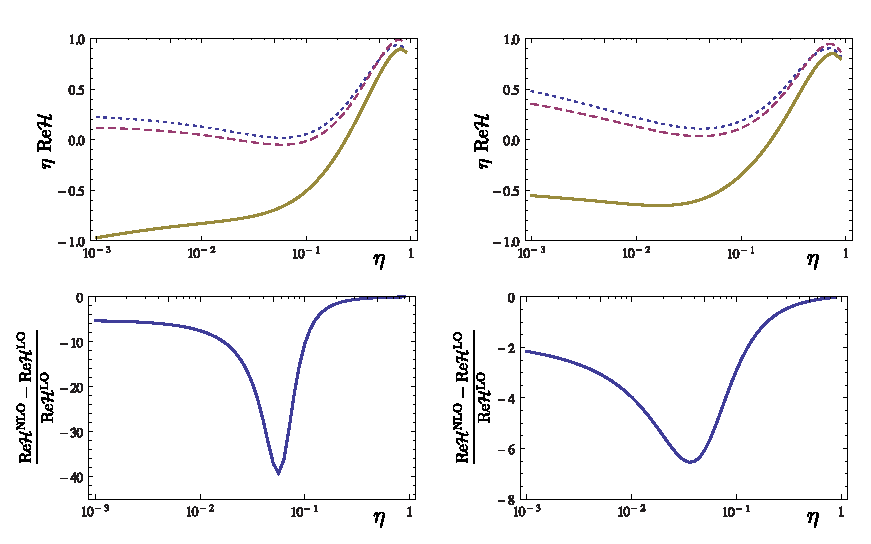
\includegraphics[width= 0.85\textwidth]{TCS_Re_2x2_nice.eps} 
\caption{The real part of the {\it timelike} Compton Form Factor
$\mathcal{H}$ multiplied by $\eta$, as a function of $\eta$ in the double
distribution model based on Goloskokov-Kroll (upper left) and MSTW08 (upper
right) parametrizations, for $\mu_F^2=Q^2=4$~GeV$^2$ and $t=-0.1$~GeV$^2$.
Below the ratios of the NLO correction to LO result of the corresponding
models.}
\label{fig:TCSRe2x2}
\end{center}
\end{figure}
%%%%%%%%%%%%%%%%%%%%%%%%%%%%%%%%%%%%%%%%%%%%%%%%%%%%%%%%%%%%%%%%%
%%%%%%%%%%%%%%%%%%%%%%%%%%%%%%%%%%%%%%%%%%%%%%%%%%%%%%%%%%%%%%%%%%%%%%%%
\begin{figure}[ht]
\begin{center}
  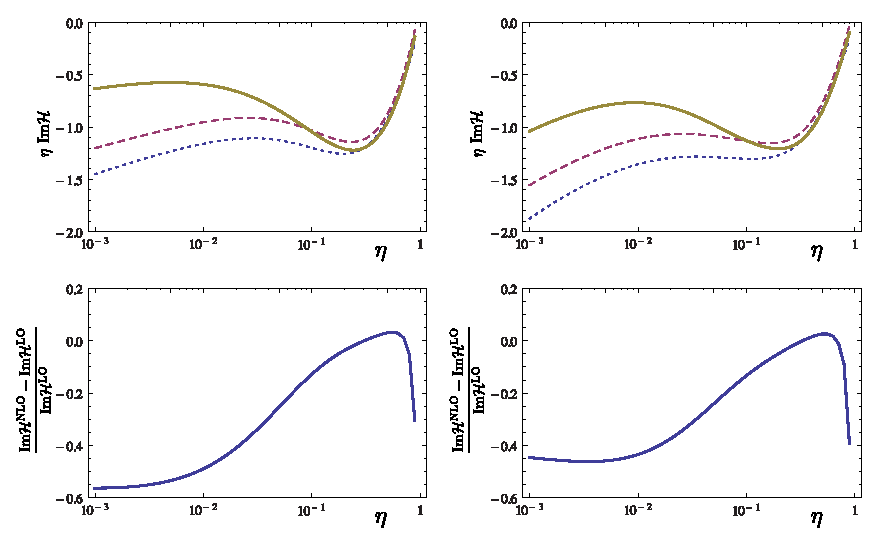
\includegraphics[width= 0.85\textwidth]{TCS_Im_2x2_nice.eps} 
\caption{The imaginary part of the {\it timelike} Compton Form Factor
$\mathcal{H}$ multiplied by $\eta$, as a function of $\eta$ in the double
distribution model based on Goloskokov-Kroll (upper left) and MSTW08 (upper
right) parametrizations, for $\mu_F^2=Q^2=4$~GeV$^2$ and $t=-0.1$~GeV$^2$.
Below the ratios of the NLO correction to LO result of the corresponding
models.}
\label{fig:TCSIm2x2}
\end{center}
\end{figure}
%%%%%%%%%%%%%%%%%%%%%%%%%%%%%%%%%%%%%%%%%%%%%%%%%%%%%%%%%%%%%%%%%
To show the importance of including NLO effects in the timelike CFFs relevant
to timelike Compton scattering, we plot in Fig.~\ref{fig:TCSRe2x2} and
Fig.~\ref{fig:TCSIm2x2}, the real and imaginary parts of the CFF $\mathcal{H}$
for the GK and the MSTW08 models of GPDs, for the invariant mass of the lepton
pair $Q'^2=4$ GeV$^2$, $t=-0.1$ GeV$^2$. For the imaginary part the correction
does not exceed $40\%$. In the real part, the correction is of the order of
few hundred percent. We observe that the main part of that large correction
comes from the contribution of gluonic GPDs. 

%\begin{figure}[ht]
%\begin{center}
%  \includegraphics[width=7cm]{ReHerr_nice.eps}  ~~~~ \includegraphics[width= 7cm]{ImHerr_nice.eps} 
%\caption{The real (left) and imaginary(right) parts of the TCS Compton Form Factor $\mathcal{H}$ multiplied by $\eta$, as a function of $\eta$ in the double distribution model based on MSTW08 parametrization, for $\mu_F^2=Q^2=4$~GeV$^2$ and $t= -0.1$~GeV$^2$. The dotted line shows the LO result and shaded bands around solid lines show the effect of a one sigma uncertainty of the input MSTW08 fit to the full NLO result.}
%\label{fig:TCSerror}
%\end{center}
%\end{figure}
%%%%%%%%%%%%%%%%%%%%%%%%%%%%%%%%%%%%%%%%%%%%%%%%%%%%%%%%%%%%%%%%%%%%


The $D$-term contribution to the CFF is a $\eta$-independent quantity and it
has both a real and an imaginary parts at NLO. 
We show in Tab.~\ref{tableDTCS} the values of this $D$-term contribution in
the LO and NLO cases. Its relative effect on the imaginary part of the CFF
decreases significantly when $\eta$ decreases, from 10 to 1 and 0.1\% when
$\eta$ decreases from 0.1 to 0.01 and to 0.001.
%Table
\begin{table*}[h]
\begin{center}
\begin{tabular}{|c||c|c|}
\hline
 & Re$\mathcal{H_D}$ &  Im$\mathcal{H_D}$ \\ \hline \hline
LO &  -2.59 & 0 \\ \hline
NLO quark contribution & -0.16 & -0.85 \\ \hline
NLO gluon contribution & 0.18 & 0.16 \\ \hline
Full NLO & -2.57 & -0.69 \\ 
\hline
\end{tabular}
\caption{\small Different contributions to the $D$-term. The values of the
real part coincides for spacelike and timelike CFF $\mathcal{H}$, while the
imaginary part is non-vanishing only for the timelike case.}
\label{tableDTCS}
\end{center}
\end{table*}

We then compare TCS and DVCS by plotting the ratio of NLO corrections on
Fig.~\ref{fig:TCStoDVCS}. There is a striking difference in the magnitude of
the corrections to the real part of CFFs, mostly insensitive to the choice of
GPD parametrizations. As discussed in Ref.~\cite{Muller:2012yq}, this is a
consequence of Eq.~(\ref{eq:TCSvsDVCS}) which by adding a phase to the
dominant imaginary part of the spacelike CFF at small skewness, gives rise
to a sizeable real part of the corresponding CFF in the timelike case.
Such large corrections to the real part of CFFs will have a significant
influence on observables which depend on the interference of the TCS process
with the Bethe-Heitler amplitude, {\sl i.e.} connected to the azimuthal
angular distribution of the leptons. 
\begin{figure}[ht]
\begin{center}
  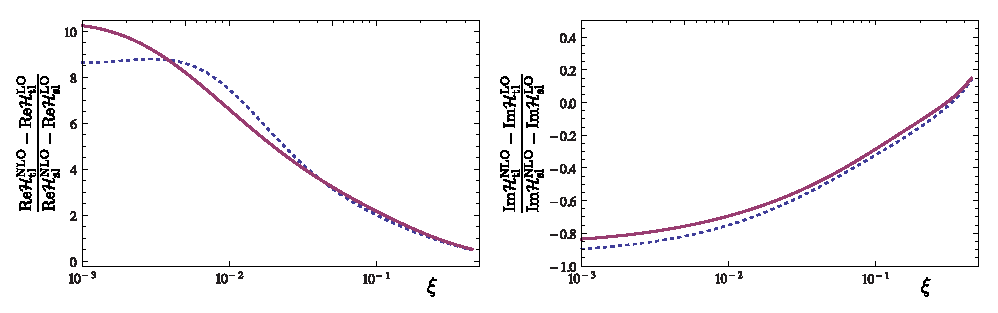
\includegraphics[width= 0.85\textwidth]{TCStoDVCS_1x2_nice.eps}
\caption{The ratio of the timelike to spacelike NLO corrections in the real
(left) and imaginary (right) part of the Compton Form Factor $\mathcal{H}$,
as a function of $\xi$ in the double distribution model based on the
Goloskokov-Kroll (dashed) and MSTW08 (solid) parametrizations, for
$\mu_F^2=Q^2=4$~GeV$^2$ and $t= -0.1$~GeV$^2$. For comparison timelike CFFs
where calculated at $\eta = \xi$.}
\label{fig:TCStoDVCS}
\end{center}
\end{figure}


\subsubsection{Cross sections and asymmetries}
Let us now pass to our estimates for the observables in TCS. Generally we
observe that the inclusion of the NLO corrections is more important at small
skewness. We also see that the Bethe-Heitler dominates the integrated
cross-section for this kinematics. In consequence, more differential
observables, as the azimuthal $\phi$ dependence (with angles $\theta$ and
$\phi$ defined in Ref.~\cite{Berger:2001xd}) reveal in a better way the
different contributions. Moreover simple $\phi$ dependence of the interference
term allows for an easy access to the real part of the CFFs which, as we
observed in Fig.~\ref{fig:TCSRe2x2}, is subject to big NLO corrections. We
indeed observe that effect on the Fig.~\ref{fig:xsec_phidep}, which shows the
$\phi$ dependence of the unpolarized differential cross sections for pure BH
process, and with a LO and NLO corrections to the interference term.
%
\begin{figure}[ht]
\begin{center}
%\epsfxsize=0.8\textwidth
 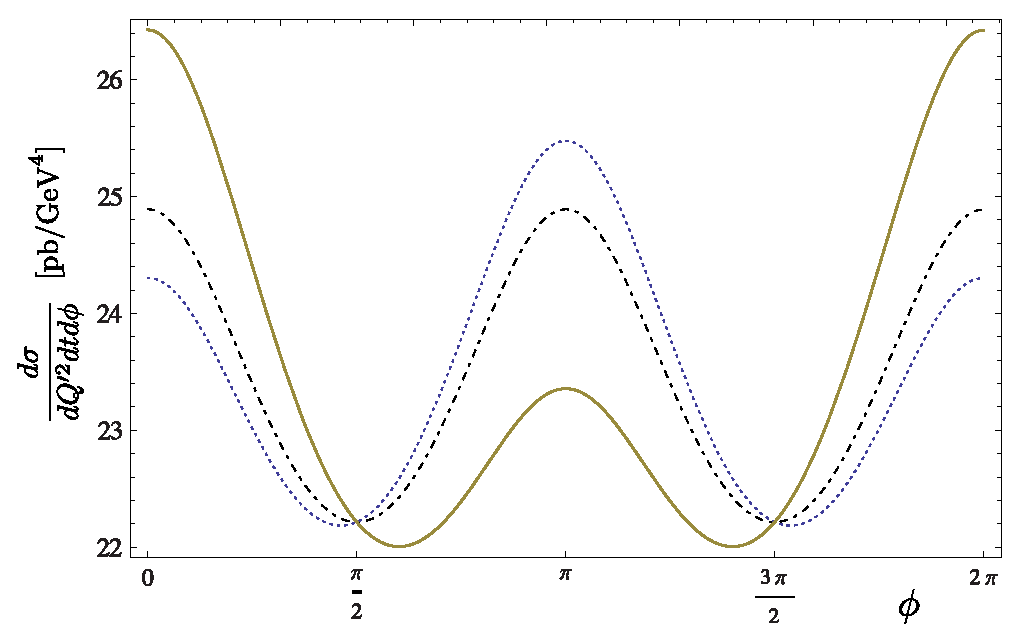
\includegraphics[width=8 cm]{xsec_phidep.eps}
\caption{The $\phi$ dependence of the cross-section at $E_\gamma = 10$ GeV,
 $Q^2 = \mu_F^2 = 4$~GeV$^2$, and $t= -0.1$~GeV$^2$ integrated over $\theta
\in (\pi/4,3\pi/4)$: pure Bethe-Heitler contribution (dash-dotted),
Bethe-Heitler plus interference contribution at LO (dotted) and NLO (solid).}
\label{fig:xsec_phidep}
\end{center}
\end{figure}

\begin{figure}[ht]
\begin{center}
%\epsfxsize=0.8\textwidth
  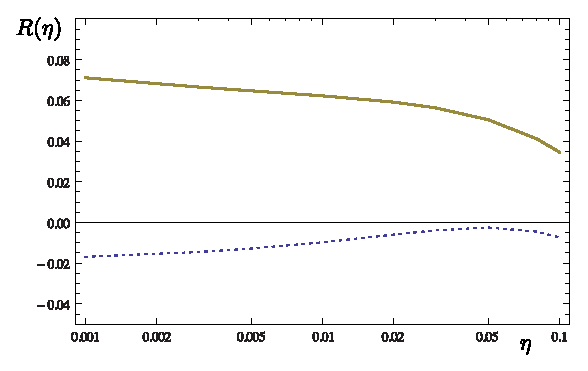
\includegraphics[width=8 cm]{R.eps}
\caption{Ratio R defined by Eq.~(\ref{eq:R_ratio}) as a function of $\eta$,
for $Q^2 = \mu_F^2 = 4$~GeV$^2$ and $t= -0.1$~GeV$^2$. The dotted line
represents LO contribution and the solid line represents NLO result.}
\label{fig:Ratio_R}
\end{center}
\end{figure}


%\begin{equation}
%\frac{
%\frac{d\sigma}{dQ'^2dtd\varphi}\left(\phi=0\right)
%-\frac{d\sigma}{dQ'^2dtd\varphi}\left(\phi=\pi\right)
%}
%{
%\frac{d\sigma_{BH}}{dQ'^2dtd\varphi}\left(\phi=0\right)
%}\,.
%\label{eq:Ratio_INT_BH_xi}
%\end{equation}

To quantify how big the deviation is from the pure Bethe-Heitler process in
the unpolarized cross section we calculate (see Fig.~\ref{fig:Ratio_R}) the
ratio R, defined in Ref.~\cite{Berger:2001xd} by
\begin{equation}
R(\eta) =  \frac{2\int_0^{2 \pi} d \varphi \,\cos \varphi\, \frac{dS}{dQ'^2dtd\varphi}}{\int_0^{2 \pi} d \varphi\frac{dS}{dQ'^2dtd\varphi}}
\,,
\label{eq:R_ratio}
\end{equation}
where $S$ is a weighted cross section given by Eq.~(43) of
Ref.~\cite{Berger:2001xd}.
It is plotted in Fig.~\ref{fig:Ratio_R} as a function of the skewness $\eta$
for $Q^2 = \mu^2 = 4$~GeV$^2$, and $t= -0.2$~GeV$^2$. In the leading twist the
numerator is linear in the real part of the CFFs, and the denominator, for the
kinematics we consider, is dominated by the Bethe - Heitler contribution. The
inclusion of NLO corrections to the TCS amplitude is indeed dramatic for such
an observable and includes also change of sign.

%This have a consequence also for the ratio $R$ defined by eq.\ref{Eq:DD}ref{RRatio}. That ratio calculated for the same kinematical region is equal on the leading order to $R_{LO} = -0.04 $ and on the next-to-leading $R_{NLO} = 0.06$.

%%%%%%%%%%%%%%%%%%%%%%%%%%%%%%%%%%%%%%%%%%%%%%%%%%%%%%%%%%%%%%%%%%%%%%%%


Imaginary parts of the CFFs are accessible through observables making use of
photon circular polarizations \cite{Berger:2001xd}. The photon beam circular
polarization asymmetry
\begin{equation}
A= \frac{\sigma^+ - \sigma^-}{\sigma^+ + \sigma^-}\,,
\end{equation}
is shown on the left part of Fig.~\ref{fig:Asymmetry_xi}, as a function of
$\phi$ for the kinematic variables relevant for JLab:
$Q^2 =4$~GeV$^2$= $\mu_F^2$, $t=-0.1$~GeV$^2$ and $E_\gamma = 10$~GeV (which
corresponds to $\eta \approx 0.11$). The same quantity is shown on the right
panel of Fig.~\ref{fig:Asymmetry_xi} as a function of $\eta$ for
$\phi = \pi/2$ and $Q^2 =4$~GeV$^2$= $\mu_F^2$. The effect of the NLO
corrections on that observable is rather large, around $10\%$ in the $\eta$
range most relevant for JLab kinematics.

\begin{figure}[ht]
\begin{center}
%\epsfxsize=0.8\textwidth
  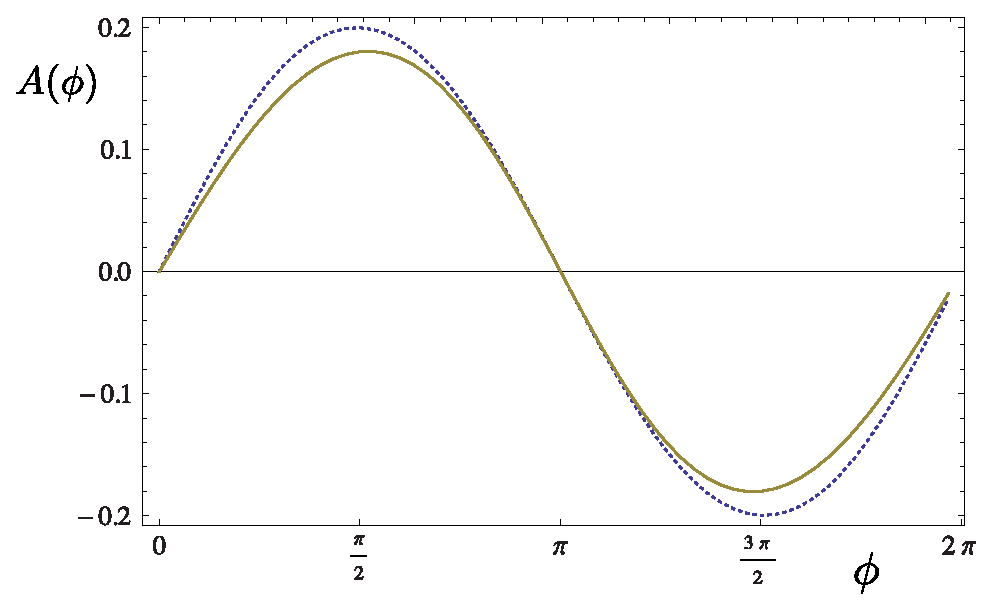
\includegraphics[width=0.4\textwidth]{Asymmetry_E_10_t_01_Q_2_nice.eps}
  \hspace{0.05\textwidth}
  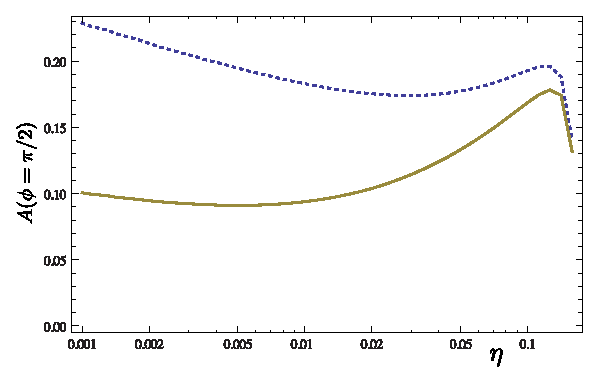
\includegraphics[width=0.4\textwidth]{Asymmetry_xi_nice.eps}
\caption{
(Left) Photon beam  circular polarization asymmetry as a function of $\phi$,
for $t=-0.1$~GeV$^2$, $Q^2 = \mu_F^2 = 4$~GeV$^2$, integrated over $\theta
\in (\pi/4,3\pi/4)$ and for $E_\gamma = 10$~GeV ($\eta \approx 0.11$).
(Right) The $\eta$ dependence of the photon beam circular polarization
asymmetry for $Q^2 = \mu_F^2 = 4$~GeV$^2$, and $t= -0.2$~GeV$^2$ integrated
over $\theta \in (\pi/4,3\pi/4)$. The LO result is shown as the dotted line,
the full NLO result by the solid line.}
\label{fig:Asymmetry_xi}
\end{center}
\end{figure}
